The bare-minimum multirotor remote-piloted aerial system (RPAS) or informally referred as ``drone'', consists of a propulsion system, flight controller, speed controllers, battery/fuel, and sensor systems.

\subsubsection{Multirotor Configuration}

A multirotor RPAS (MRPAS) has several common configurations: a tricopter, a quadcopter, and a hexacopter such as seen in figure \ref{fig:mrpas-config} below.

\begin{figure}[H]\label{fig:mrpas-configs}
    \centering
    \begin{subfigure}[b]{0.3\textwidth}
        \centering
        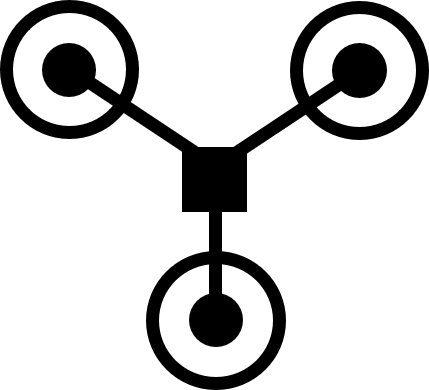
\includegraphics[scale=0.4]{img/drone_yconfig}
        \caption{Tricopter Y-Configuration}
        \label{fig:tricopter-y}
    \end{subfigure}
    ~
    \begin{subfigure}[b]{0.3\textwidth}
        \centering
        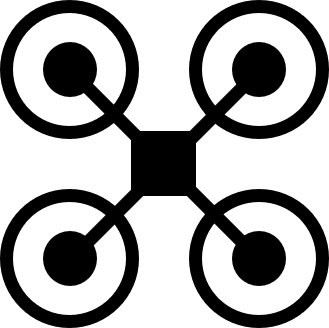
\includegraphics[scale=0.4]{img/drone_xconfig}
        \caption{Quadcopter X-Configuration}
        \label{fig:quadcopter-x}
    \end{subfigure}
    ~
    \begin{subfigure}[b]{0.3\textwidth}
        \centering
        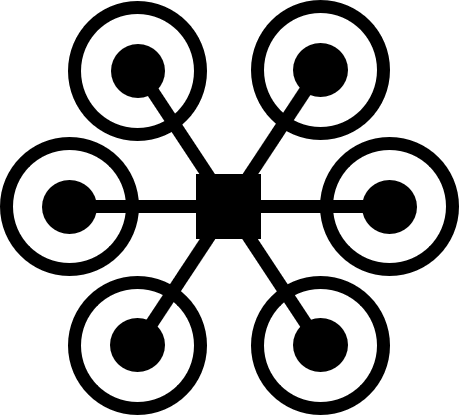
\includegraphics[scale=0.4]{img/drone_hexconfig}
        \caption{Hexcopter X-Configuration}
        \label{fig:hexcopter-x}
    \end{subfigure}
    
    \caption{Multirotor RPAS Configurations}
    \label{fig:rpas_configs}
\end{figure}

\textbf{Tricopter: } Tricopters requires fewer motors and speed controllers, implying less components and power draw required to sustain flight. The angle between each motor arm is also wider at 120 degrees and thus reduces obstruction from camera views. 

\begin{figure}[h]
    \centering
    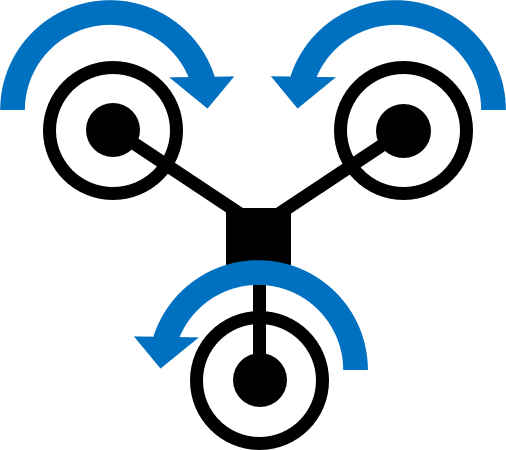
\includegraphics[scale=0.4]{img/drone_yconfigt}
    \caption{Tricopter Y-configuration}
    \label{fig:tricopter-y-t}
\end{figure}

However, systems with odd-number of actuatators are inherently unstable due to the asymmetry of the motor torque as shown in figure \ref{fig:tricopter-y-t}. Therefore, this design require an additional servo motor (consists of a DC motor and a gear box) to precisely control the tail motor angle of tilt to counter the excess torque --- similar to the tail of a helicopter.

We choose to not pursue this configuration as the tricopter configuration provides agility with require increased control complexity as a trade off. This compromise is not ideal as we emphasize on flight stability.

\textbf{Quadcopter X: }
The quadcopter is the most common configuration in consumer multirotor products. The quadcopter is more stable than a tricopter because a quadcopter configuration utilizes four motors as seen in Figure \ref{fig:quadcopter-x-t}. Two of the motors spin clockwise and the other two spin counter-clockwise and effectively cancelling each other’s undesired torque. Applying the same power into each motor allows the MRPAS to hover in place. We can perform 6 degree-of-freedom (DOF) movements by changing a combination of differential thrust to each motor (Figure \ref{fig:rpas_6dof}).

\begin{figure}[H]
    \centering
    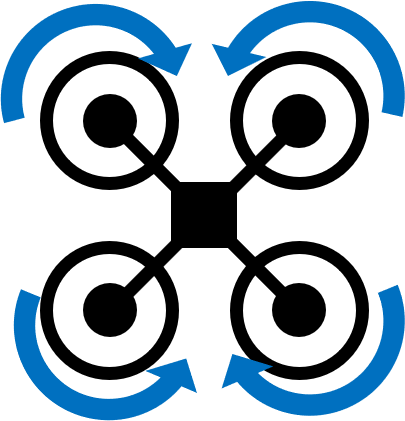
\includegraphics[scale=0.4]{img/drone_xconfigt}
    \caption{Quadcopter X-configuration}
    \label{fig:quadcopter-x-t}
\end{figure}

\begin{figure}[H]
    \centering
    \begin{subfigure}[b]{0.3\textwidth}
        \centering
        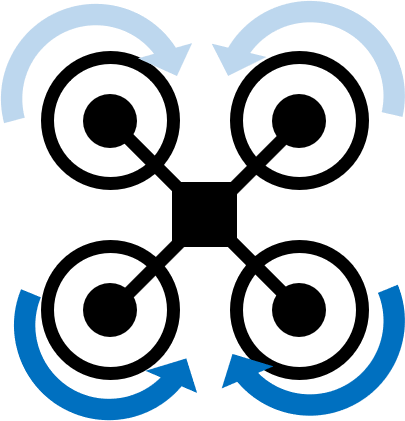
\includegraphics[scale=0.4]{img/drone_x_pitch}
        \caption{Pitch forward}
        \label{fig:x-pitch}
    \end{subfigure}
    ~
    \begin{subfigure}[b]{0.3\textwidth}
        \centering
        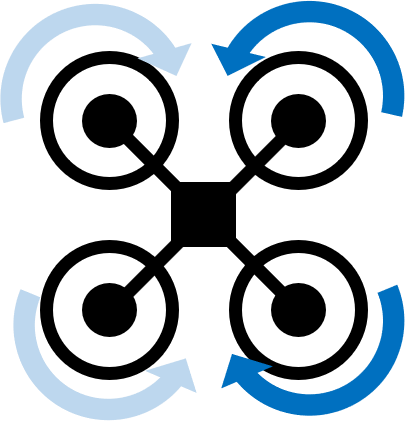
\includegraphics[scale=0.4]{img/drone_x_roll}
        \caption{Roll left}
        \label{fig:x-roll}
    \end{subfigure}
    ~
    \begin{subfigure}[b]{0.3\textwidth}
        \centering
        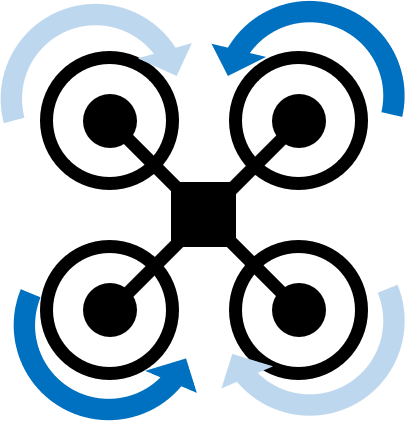
\includegraphics[scale=0.4]{img/drone_x_yaw}
        \caption{Yaw left}
        \label{fig:x-yaw}
    \end{subfigure}
    
    \caption{Using differential thrust to obtain 6-DOF movement. }
    \label{fig:rpas_6dof}
\end{figure}

\textbf{Hexacopter X: }
The hexacopter has all the stability benefits of a quadcopter as well as extra redundancy. The MRPAS could still land safely even up to dual motor failures. Since the hexacopter uses two more motors than the quadcopter configuration, naturally, the RPAS of this configuration is generally bigger and can lift more payload. Of course, with the added components, it is also much more expensive to build, operate, and maintain. Furthermore, hexacopter RPAS's extended size and mass can cause more damage upon a crash.

We choose to the quadcopter configuration. 
The payload is not too heavy -- our target maximum payload weight is less than 500 g (\textbf{NF.DR.1}). The quadcopter configuration is also the most balanced in terms of the trade-off between cost and reliability. 

\subsubsection{Air Frame}\label{section:air-frame}

The most common frame available for sale comes in 450 mm motor to motor diagonal span (MMDS) variants. However, 
350mm is also common amongst consumer products, such as DJI Phantom. The problem with 350 mm is that it will 
constrain our ability to mount larger hardware such as the computing platform. The 350 mm also limits 
propeller size. On the other hand, the largest quadcopter configuration has an MMDS of 650 mm or 1000 mm 
to allow for extremely large payload capacity. However, these are more commonly used for industrial or military 
applications.

\begin{figure}[H]
    \centering
    \begin{subfigure}[b]{0.33\textwidth}
        \centering
        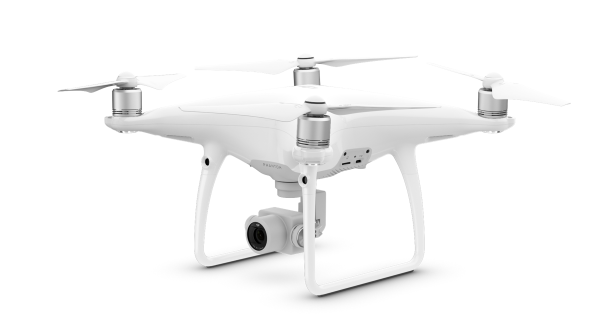
\includegraphics[width=\textwidth]{img/djiphantom4}
        \caption{DJI Phantom 4 (350 mm)}
    \end{subfigure}
    ~
    \begin{subfigure}[b]{0.33\textwidth}
        \centering
        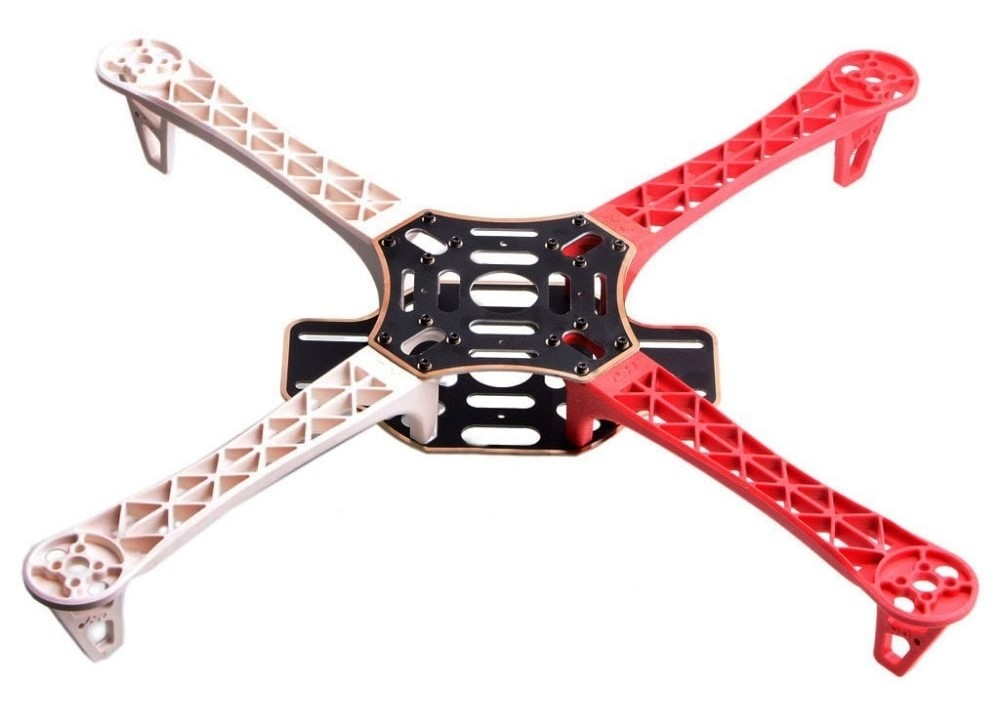
\includegraphics[width=\textwidth]{img/f450frame}
        \caption{Generic DIY frame kit (450 mm)}
    \end{subfigure}
    ~
    \begin{subfigure}[b]{0.33\textwidth}
        \centering
        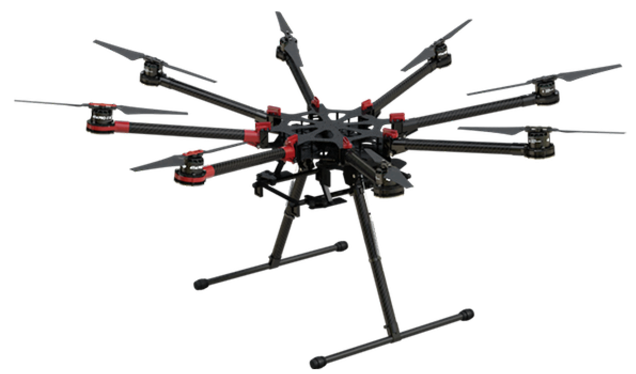
\includegraphics[width=\textwidth]{img/djis1000}
        \caption{DJI Spreadwings S1000 (1000 mm)}
    \end{subfigure}
    
    \caption{Air Frame Sizing Options }
\end{figure}

We chose a frame size of 450 mm MMDS which has a good balance between portability and capability. The 450 mm frames 
can accommodate larger propellers and are the 
most abundant size on the market for frames due to their versatility and are therefore less costly 
and easy to repair/replace.

Currently, the \textit{Upgrade F450} for CA\$30.00 and \textit{Diatone Q450} for CA\$20.00 from \textit{Banggood} are appealing options. They weigh between 300 g to 410 g, which are both acceptable.

\subsubsection{Propulsion System}

The propulsion system covers the majority of the RPAS parts list and determines the flight performance of the RPAS. 

\paragraph{Motor Type}

The MRPAS is electrically powered with a battery (DC). Thus, we have two options for motors: DC brushed 
motors and DC brushless motors.

Brushed motors use mechanical brushes in contact with rotor’s commutator to switch polarity to sustain a 
constant rotation, whereas the brushless motors use electronic controllers to switch the polarity in the 
rotor electrically. 

For flight applications, we chose the brushless DC (BLDC) motors for their extended usable life time. 
BLDC motors are also much more efficient than brushed motors because as they do not mechanically swap 
the polarity in the motor, which results in excess friction, heat, and potential sparking.

BLDC motors are further broken down into two types: in-runner and out-runner. In-runner motors have the rotor 
on the inside and the out-runner motors have the rotor on the outside. We chose out-runner because they’re 
commonly used for multirotor RPAS systems. The out-runner solution also comes with benefits: as the rotor is on the 
outside, heat dissipation is significantly more efficient. Since the rotating mass is further from the 
center of rotation for an out-runner, the rotational inertia helps to stabilize the angular momentum of the 
rotor. Of course, this means that the out-runner has a slower spin-up time than the in-runner, but for a 
multirotor RPAS typically operating in stabilized flight and hover, the agility of an in-runner is not 
practical.

\paragraph{Motor Size and Speed}\label{section:motor-speed}

All BLDC out-runner motors have the same height, and on product pages they are often given the code 22XX to denote their stator size. The design parameter is the radius (XX on the product code). Typically, the larger the stator (radius), the slower it spins given the same voltage. This is a linear relationship described by the motor parameter kV:

$$
\omega_{\mathrm{RPM}} = \mathrm{kV} \times \mathrm{Voltage}
$$

The kV constant is inversely proportional to another motor constant, kT, which models the linear relationship between current and torque:

$$
\tau = \mathrm{kT} \times \mathrm{Current}
$$

The inverse relationship can be shown by equating electrical power into the motor and mechanical power produced by the motor:

$$
\tau\omega_{\mathrm{RPM}} = \mathrm{kV}\mathrm{kT}\times VI
$$

By constraining the electrical power, we can make trade-off between torque and rotation speed.
Air resistance (“drag”) is proportional to speed of an object squared, therefore the power required to 
lift increases non-linearly to the force output. As seen in the test data obtained from one manufacturer’s 
datasheet below, when using the same propellers we see an increased thrust output resulting from increased voltage (and 
thus current). However the efficiency, typically measured in g/W, decreases. 

Below is a sample set of thrust output using a SunnySky X2216 1250 kV motor using 9.0 inch 5.0 inch pitch and 10.0 inch 4.7 inch pitch propellers obtained from a vendor website \cite{sunnysky-2216}. 

\begin{table}[H]
    \centering
    \caption{Sample Motor Test Data}
    \label{table:sunnyskyx2216-table}

    \begin{tabular}{lrrrrr}

    \hline
    \textbf{Propeller} & \textbf{Voltage} & \textbf{Current} & \textbf{Pull}  & \textbf{Power Consumption} & \textbf{Efficiency}\\
    & [V] & [A] & [g] & [W] & [g/W] \\
    \hline
     & 10.0 & 16.4 & 940 & 164 & 5.73 \\
    9050 & 11.0 & 19.5 & 1050 & 215 & 4.89 \\
     & 12.0 & 21.5 & 1250 & 258 & 4.84 \\
    \hline
     & 10.0 & 23.5 & 1200 & 235 & 5.10 \\
    1047 & 11.0 & 26.5 & 1350 & 372 & 3.63 \\
     & 12.0 & 30.2 & 1520 & 363 & 4.19 \\
    \hline

    \end{tabular} 
\end{table}

Therefore, it makes sense that we choose larger motors with relatively lower kV constants. Slower motors 
are also safer since there is less angular momentum of the blades. Motors with 800 kV to 1300 kV are 
suitable for our applications and achieve reasonable thrust output with adequate efficiency. 2212, 2214, 
and 2216 stator sizes are suitable in this range of kV.

\paragraph{Propeller Material}

Common RPAS propellers are constructed using either plastic or carbon composite. Plastic is cheap, abundant, 
and relatively flexible. Due to their cheapness, however, their manufacturing is not as precise, leading to 
aerodynamic inefficiencies. Plastic propellers often require balancing where tape is applied to one of the 
blades such that the weight is balanced---minimizing vibrations. Carbon composite propellers, such as 
carbon fibre blades, are extremely light and subsequently much more expensive. The carbon composite 
propellers have micro-meter precision manufacturing, however, providing top efficiency. Carbon composite 
propellers are not flexible and extremely tough. It is more dangerous for persons to be near spinning 
carbon composite propellers due to their sharpness and toughness, and could lead to serious injuries or death.

Due to budget constraint and safety concerns, we chose plastic propellers.

\paragraph{Propeller Size and Pitch}

\textbf{Notation: } Propeller size and pitch is commonly denoted by RRYY where RR is the propeller diameter in inches, and YY is the propeller pitch in degrees. (9050 denotes a propeller with 9 inch diameter, and 5.0 inches of pitch; 1045 denotes a propeller with 10 inch diameter, and 4.5 inches of pitch).

\begin{figure}[H]
    \centering
    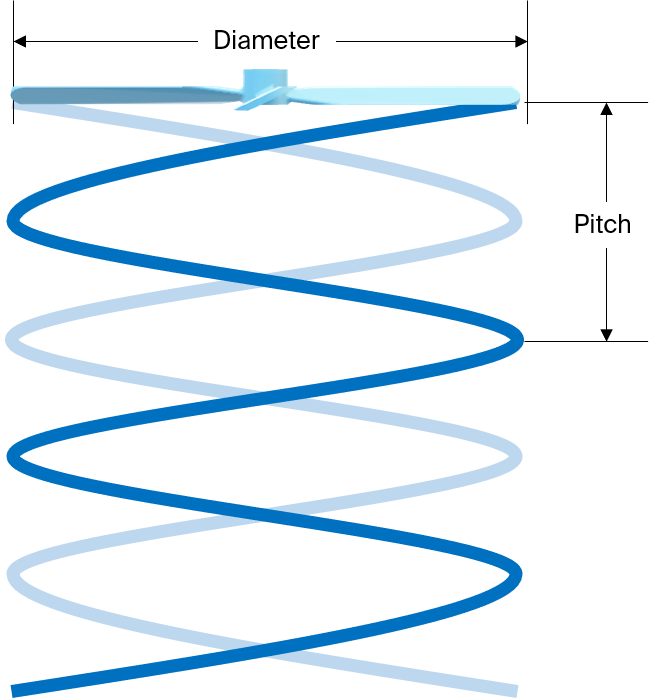
\includegraphics[scale=0.5]{img/proppitch}
    \caption{Propellor Diameter and Pitch Parameters}
    \label{fig:propeller}
\end{figure}

To obtain maximum thrust with low speed (low speed is more desirable, as mentioned in Section \ref{section:motor-speed}), we want to choose the biggest possible propeller diameter.

\begin{figure}[H]
    \centering
    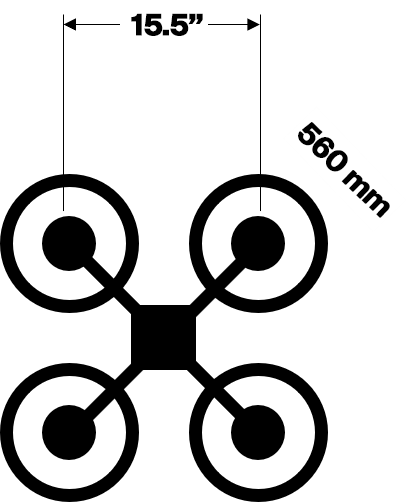
\includegraphics[scale=0.5]{img/framepropsize}
    \caption{Maximum Propeller Sizes}
    \label{fig:framepropsize}
\end{figure}

As mentioned in Section \ref{section:air-frame}, we chose the 450 mm frames, which means that the motor to motor 
adjacent span (MMAS) is about 12.5 inches. It is safe to provide 1 inch of clearance between propellers, 
therefore the ideal size of propellers to choose is 10 or 11 inches.

Mentioned in Section \ref{section:motor-speed}, we chose low-speed motors for their efficiency. And recall that 
given the same power: a slow-speed motor provides inversely proportional torque, so we chose propellers 
with relatively high pitch (between 3 to 5 inches) to take advantage of the high-torque output and to
maximize thrust output.

Here is a list of desirable propeller size and pitches: 1030, 1045, 1130, 1145.

\paragraph{Speed Controllers}

The electronic speed controller (ESC) controls the voltage and current supplied to a BLDC motor. All ESCs 
function identically and the design parameters are size/weight, rating, efficiency, and cost.

As shown in Table 2, the typical maximum current draw is approximately 30 A. For a 
safety margin of 10 A, we decided to select ESCs with maximum rating of 40 A. All of the following options are appealing:

\begin{table}[H]
    \centering
    \caption{ESC Purchasing Options}
    \label{table:esc-table}

    \begin{tabular}{lrrrll}

    \hline
    \textbf{ESC} & \textbf{Rating} & \textbf{Weight} & \textbf{Price}  & & \textbf{Vendor}\\
    & [A] & [g] & [CA\$] & & \\
    \hline
    HAKRC BLHeli Dshot1200 & 35 & 7  & 40.00 & per 4 & Banggood\\
    Racestart RS30A Lite & 30 & 6  & 40.00 & per 4 & Banggood\\
    Racestart SPROG X DShot600 & 35 & 4  & 30.00 & per 4 & Banggood\\
    Skystars Talon32 & 40 & 7  & 12.00 & per 1 & Banggood\\
    \hline

    \end{tabular} 
\end{table}

\subsubsection{Flight Controller}

Flight controllers (FC) come in different tiers differentiated by their price and features. 

The cheapest FC typically only has the bare-minimum features for flight (such as accelerometers and 
self-hover functions). These flight controllers are typically designed for acrobatic or basic VLOS 
flying and typically cost CA\$20 to CA\$50. The firmware that runs on these FCs are typically 
open-source but nonetheless user-friendly and easily-programmable. Below is a list of FCs which falls 
under this tier:

\begin{itemize}[noitemsep,topsep=0pt, parsep=4pt, partopsep=0pt]
    \item F1, F3, F4, F7 FC are minimal in weight and footprint; they are ideal for light-weight operations.\cite{f1fc}
    \item KK 2.15 FC features a built-in display on the board, allowing quick access to flight settings without the need to connect to a computer for reprogramming.
    \item Naze32 FC is reliable with auto-tuning PIDs.
    \item CC3D FC is reliable with auto-tuning PIDs.
\end{itemize}

The next tier of FCs have more advanced features such as GPS-hold, autonomous flight, anto-land, 
telemetry, etc. They are designed for more advanced operation. These FCs are more expensive, costing 
CA\$50 to CA\$200, however these FCs have excellent after-sale support for their respective 
manufacturers and their documentation is better. Along 
with frequent manufacturer firmware updates, the mid-tier FCs are more reliable. The downside is that 
they are typically heavier and take up a much larger footprint. 
Below is a list of mid-tier FCs:

\begin{itemize}[noitemsep,topsep=0pt, parsep=4pt, partopsep=0pt]
    \item ArduPilot APM 2.8 is a flight controller using Arduino Mega and supports GPS and telemetry.
    \item Pixhawk PX4 Autopilot features pre-programmable autonomous operations.
    \item DJI Naza M Lite.
\end{itemize}

For the applications we require, we chose the ArduPilot APM 2.8 as it is the most flexible option with advanced features at a reasonable price of CA\$75.00. Additionally, due to of the low-cost of low-tier FCs, we will also purchase one of the Naze32 or CC3D FC modules as a back-up.

\subsubsection{Radio Systems}

The minimum number of channels required to fly a drone is 4 -- one for each control: throttle, yaw, 
pitch, and roll. For this reason, we opted for the cheapest radio transmitter (TX) and receiver  (RX) 
combo we found from online vendors. 
The FlySky-FS i6 2.4GHz 6-Channel TX and RX bundle is ideal for our application due to its low cost.
According to the FlySky-FS i6 datasheet\cite{flyskyi6}, the radio frequency (RF) peak power is below 20 dBm while still achieving a maximum control range of 500 m (\textbf{NF.DR.4}).

\subsubsection{Battery}

We chose lithium polymer (Li-Po) batteries as they have the highest energy density (highest capacity to weight ratio) similar to that of lithium-ion (Li-ion) batteries, and thus are perfect for high-power, low-weight applications. Figure~\ref{fig:batterytypes} shows a graph of energy density of types of batteries \cite{battery} --- from this graph, it is clear that Li-Po batteries are to be chosen.

\begin{figure}[h]
    \centering
    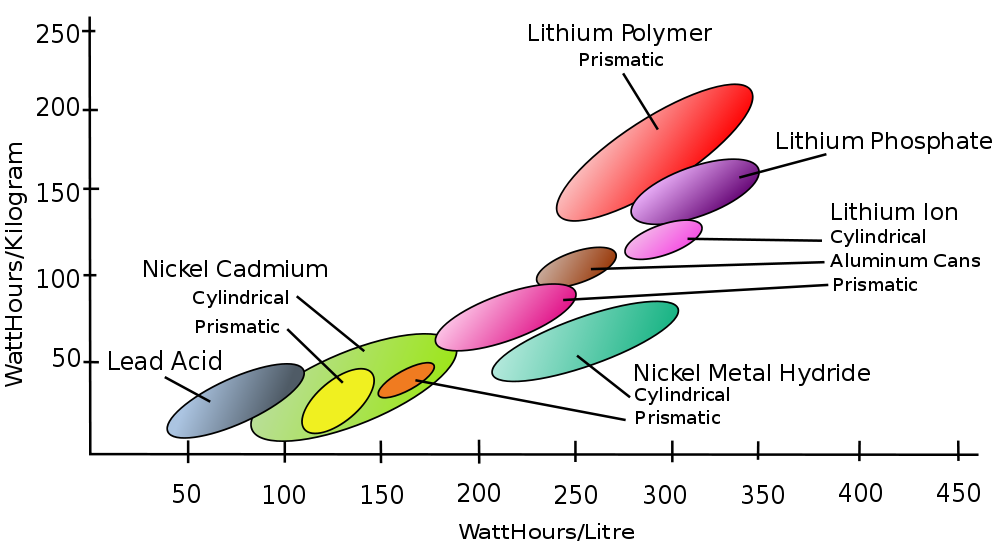
\includegraphics[scale=0.5]{img/energydensity.png}
    \caption{Energy Density Graph of Various Battery Types}
    \label{fig:batterytypes}
\end{figure}

Li-Po batteries have mainly three design parameters: configuration, capacity,  discharge rating, and internal resistance.

\textit{Configuration} is how the Li-Po batteries are manufactured and wired together: a single cell in a Li-Po battery provide a 
nominal voltage of 3.7 V due to its electrochemistry.
Similar to how portable electronics and appliances require AA or AAA batteries placed in a certain order, a single cell of 3.7 V is not enough to drive anything powerful. Ergo multiple cells can be wired in series and the 
voltage adds up: 2 cells in series, denoted by ``2S'' batteries have 7.4 V output, 3S batteries have 11.1 V output, and 4S batteries have 14.8 V output. 

Battery \textit{capacity} is measured in watt-hours (Wh) or milli-amp-hours (mAh), which is unit of electric power multiplied by unit time. A 20.0 Wh battery can output 20.0 W for 1.0 hour. Multiple battery cells can be put in parallel and their capacity adds up. A pair of four-cell batteries wired in parallel, denoted by ``4S2P'' have a 14.8 V output while double the capacity of a single 4S battery of the same variant.

The \textit{discharge rating} is denoted by ``C'' and indicates the ratio of he capacity and maximum discharge current safely without significantly harming the battery's life. A 1,000 
mAh battery with a discharge rating of 20 C can discharge a maximum of 1.0 A $\times$ 20 C = 20 A. It is important to note that a high discharge rating does not imply improved performance, but the \textitt{internal resistance}. Since a higher internal resistance means that the battery can run less efficiently with power lost internally\cite{battery-c}. In reality, the internal resistance is merely a value on the data-sheet and not a design parameter --- thus we will choose the battery with the most optimal internal resistance as alotted by our budget. 

We will choose the design parameters for the battery after we have consolidated on the rest of the parts for the RPAS -- allowing for more system flexibility.
